En este pasaje se habla sobre el diagrama de estados del sistema. El objetivo de este consiste en representar el funcionamiento de la lógica que se encuentra en Node-Red.

Cabe aclarar que por cuestiones de practicidad, en la Imagen (\ref{fig:diagrama_de_estados}) se simbolizan con nodos rojos, la interacción que el usuario tenga con la interfaz gráfica. Estos nodos representan los datos que se ingresan en el servidor por parte del cliente. Es decir, una comunicación unidireccional de la persona hacia el nido.

\begin{figure}[H]
	\centering	
	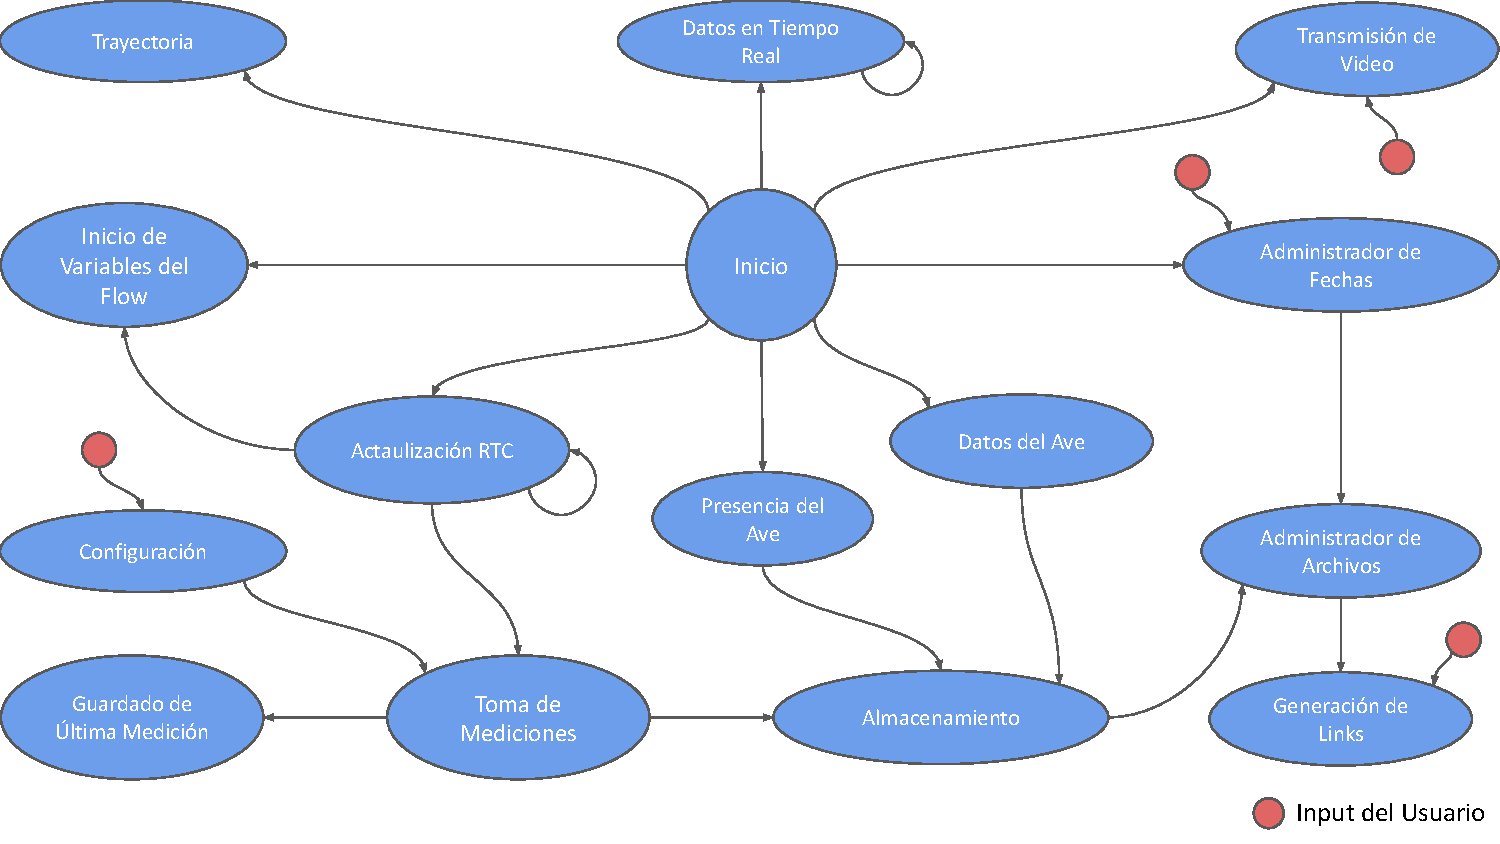
\includegraphics[width=\textwidth, page=1]{ImagenesIngenieria de Detalle/FlowChartNodeRed.pdf}	
	\caption{Diagrama de estados.}
	\label{fig:diagrama_de_estados}
\end{figure}

El nodo \textit{Inicio} es el principal. Si bien es el más simple, es el más importante porque inicia todo el sistema y su configuración. Este estado se ocupa de mandar distintos tipos de señales de arranque. Estas varían dependiendo del tipo de inicio que se busca determinar, distinguiendo así tres versiones distintas:
\begin{itemize}
	\item \textit{Init:} esta señal se envía cuando se inicia el servidor o cuando se realiza un cambio en los nodos mediante el usuario de administrador.
	\item \textit{F5:} se envía esta indicación cuando el usuario actualiza la página a la que tiene acceso.
	\item \textit{Init And F5:} esta es una combinación de las dos anteriores. El objetivo de esta es simplificar el esquema del sistema al momento de conectar los distintos estados y manejar su comunicación.
\end{itemize}

El siguiente estado en cuando a importancia es el de \textit{Actualización RTC}. Este es un nodo que se ocupa de leer el periférico de RTC y actualizar el valor dentro de Node-Red de manera periódica.

Con una de sus salidas se ocupa de inicializar las demás variables que se emplean en el servidor llamando a \textit{Inicio de Variables del Flow}. Es importante aclarar que las variables del flow son del tipo globales, es decir, cada nodo puede leerlas y modificarlas. Por cuestión de orden se asignó un estado propio para asignar valores por defecto y garantizar un correcto funcionamiento desde el arranque.

Con la salida faltante se comunica con el estado de \textit{Toma de Mediciones}. Como su nombre lo indica, se ocupa de verificar si ha transcurrido el intervalo de tiempo requerido con respecto a la última medición realizada. En caso afirmativo, se realiza la medición y luego informa a \textit{Guardado de Última Medición}, el cual actualiza la fecha y hora de este dato. Si bien \textit{Inicio de Variables del Flow} configura un intervalo por defecto para cada variable, \textit{Configuración} brinda la posibilidad de que el usuario cambie esos intervalos, manteniéndose en un margen de entre 5 minutos a 1 hora.

Con otra de las salidas del estado de \textit{Toma de Mediciones} se indica al nodo de \textit{Almacenamiento} de guardar el dato determinado. La razón por la cual \textit{Almacenamiento} tiene una salida es porque debe informar a \textit{Administración de Archivos} que hay datos nuevos. Este a su vez se ocupa de verificar cuáles de todos lo datos que posee deben ser mostrados al usuario. 

Esa decisión se encuentra regida en función de intervalos de tiempos, los cuales se determinan por una fecha inicial y final. Por defecto, \textit{Variables del Flow} asigna como día inicial y final la fecha en la cual se haya inicializado el servidor. Sumado a eso, \textit{Administrador de Fechas} se ocupa de brindarle al usuario la posibilidad de cambiar dicho período y de informar al \textit{Administración de Archivos} de dicho cambio.

El estado \textit{Generación de Links} se encarga de cargar los archivos adecuados para ser descargados y brindar al usuario acceso a estos.

\textit{Datos del Ave} obtiene los datos que se encuentran en la mochila del ave, para luego facilitárselos a \textit{Almacenamiento}. De una forma similar, \textit{Presencia del Ave} se ocupa de detectar si el ave se encuentra en el entorno del nido, mostrarlo en pantalla.

Su conexión con el estado de \textit{Almacenamiento} se da a que se guarda esta base de datos en la memoria de la R-Pi para aliviar el peso que debe soportar el servidor. Es por ello que estos a pesar de que el nodo que se ocupa de almacenar datos no brinda estos a \textit{Administrador de Archivos} ya que no es de interés que el usuario tenga acceso a la descarga de estos.

El nodo de \textit{Transmisión de Video} muestra en pantalla una transmisión en tiempo real del nido. Este se activa cuando el usuario lo solicite. Si bien es posible reiniciarlo y finalizarlo a voluntad, para evitar un uso excedido de dicha cualidad, y así evitar también una sobrecarga, el video se termina luego de 5 minutos de transmisión.

\textit{Datos en Tiempo Real} toma una medida de luminosidad, temperatura y humedad de manera periódica. Para evitar un uso excesivo de memoria, estos datos se superponen. El objetivo de este es mostrar al usuario en tiempo real las condiciones por dentro del nido.

Por último, el nodo de \textit{Trayectoria} se ocupa de mostrar la posición del ave en el entorno de medición de la red de seguimiento.